\documentclass[a4paper]{article}

\usepackage{blindtext} % Package to generate dummy text throughout this template 

\usepackage[sc]{mathpazo} % Use the Palatino font
\usepackage[utf8]{inputenc}
\usepackage[T1]{fontenc} % Use 8-bit encoding that has 256 glyphs
\linespread{1.05} % Line spacing - Palatino needs more space between lines
\usepackage{microtype} % Slightly tweak font spacing for aesthetics

\usepackage[american]{babel} % Language hyphenation and typographical rules

\usepackage[hmarginratio=1:1,top=32mm]{geometry} % Document margins
\usepackage[hang, small,labelfont=bf,up,textfont=it,up]{caption} % Custom captions under/above floats in tables or figures
\usepackage{booktabs} % Horizontal rules in tables

\usepackage[backend=biber,style=ieee]{biblatex}
\usepackage{csquotes}
\bibliography{bibliography} 

\usepackage{amsmath} 
\usepackage{amsfonts} 
\usepackage{amssymb}
\usepackage{mathtools}

\DeclarePairedDelimiter\abs{\lvert}{\rvert}

%%%%%%%%%%%%%%%%%%%%%%%%%%%%%%%%%%%%%%%%%%%%%%%%%%%%%%%%%%%%%%%%%%%%%%%%%%%%%%%
% Bilder
%%%%%%%%%%%%%%%%%%%%%%%%%%%%%%%%%%%%%%%%%%%%%%%%%%%%%%%%%%%%%%%%%%%%%%%%%%%%%%%
\usepackage{graphicx}
\usepackage{wrapfig}
\usepackage{float}
\graphicspath{{./resources/img/}}

%\usepackage{lettrine} % The lettrine is the first enlarged letter at the beginning of the text

\usepackage{enumitem} % Customized lists
\setlist[itemize]{noitemsep} % Make itemize lists more compact

%%%%%%%%%%%%%%%%%%%%%%%%%%%%%%%%%%%%%%%%%%%%%%%%%%%%%%%%%%%%%%%%%%%%%%%%%%%%%%%
% Listings
%%%%%%%%%%%%%%%%%%%%%%%%%%%%%%%%%%%%%%%%%%%%%%%%%%%%%%%%%%%%%%%%%%%%%%%%%%%%%%%
\usepackage{listings}

\usepackage[ruled, english]{algorithm2e}

\usepackage{xcolor}
\lstset{
	numbers=left,
	numberstyle=\tiny,
	numbersep=5pt,
	breaklines=true,
	showstringspaces=false,
	frame=single ,
	xleftmargin=15pt,
	xrightmargin=15pt,
	basicstyle=\ttfamily \footnotesize,
	stepnumber=2,
	captionpos=b,
	language=C,   %Sprache Festelegen
	floatplacement=H,
	tabsize=2,
	keepspaces=true
	%	keywordstyle=\color{blue},          % keyword style
	%	commentstyle=\color{dkgreen},       % comment style
	%	stringstyle=\color{mauve}         % string literal style
}


\lstdefinelanguage{scala}{
	morekeywords={abstract,case,catch,class,def,%
		do,else,extends,false,final,finally,%
		for,if,implicit,import,match,mixin,%
		new,null,object,override,package,%
		private,protected,requires,return,sealed,%
		super,this,throw,trait,true,try,%
		type,val,var,while,with,yield},
	otherkeywords={=>,<-,<\%,<:,>:,\#,@},
	sensitive=true,
	morecomment=[l]{//},
	morecomment=[n]{/*}{*/},
	morestring=[b]",
	morestring=[b]',
	morestring=[b]"""
}


\lstset{inputpath=./resources/code}



\usepackage{abstract} % Allows abstract customization
\renewcommand{\abstractnamefont}{\normalfont\bfseries} % Set the "Abstract" text to bold
\renewcommand{\abstracttextfont}{\normalfont\small\itshape} % Set the abstract itself to small italic text

\usepackage{titlesec} % Allows customization of titles
\titleformat{\section}[block]{\Large\scshape}{\thesection.}{1em}{} % Change the look of the section titles
\titleformat{\subsection}[block]{\large\scshape}{\thesubsection.}{1em}{} % Change the look of the section titles

\usepackage{fancyhdr} % Headers and footers
\pagestyle{fancy} % All pages have headers and footers
\fancyhead{} % Blank out the default header
\fancyfoot{} % Blank out the default footer
\fancyhead[C]{} % Custom header text
\fancyfoot[RO,LE]{\thepage} % Custom footer text

\usepackage{titling} % Customizing the title section

\usepackage[hidelinks]{hyperref} % For hyperlinks in the PDF
\usepackage{cleveref}
\crefname{lstlisting}{listing}{listings}
\Crefname{lstlisting}{Listing}{Listings}

%----------------------------------------------------------------------------------------
%	TITLE SECTION
%----------------------------------------------------------------------------------------

\setlength{\droptitle}{-4\baselineskip} % Move the title up

\pretitle{\begin{center}\Huge\bfseries} % Article title formatting
	\posttitle{\end{center}} % Article title closing formatting
\title{An Architecture for Embedded Graphical Interfaces} % Article title

\author{%
	\textsc{Brendan Christy} \and \textsc{Ingo Braun} \and\\[-2ex]
	\vspace{1pt} \footnotesize Department of Computer Science, University of Applied Sciences RheinMain, Germany \\ 
	\vspace{1pt} \footnotesize \texttt{\{brendan.b.christy, ingo.braun\}@student.hs-rm.de}
}

\date{\today} % Leave empty to omit a date

\renewcommand{\maketitlehookd}{%
	\begin{abstract}
		\noindent With Project AEGIS we propose an open-source hardware based graphics accelerator for low-cost embedded systems, specifically for the VexRiscv by Charles Papon. 
		Like the VexRiscv, Project AEGIS will be written in SpinalHDL, a high level synthesis library for Scala, which simplifies 
		the process of creating your own hardware, as one can use the full featureset of Scala. During the project we will be able to
		rasterize lines and circles, bliting bit graphics, and will have a core for various arithmetic operations.
		The creation of an open-source hardware based graphics accelerator has several reasons. One key factor is to have hardware sovereignity, meaning to become independent form
		hardware manufacturers. Additionaly it is also important to learn how GPUs work, since not much of the inner workings is publicised. Lastly certain
		embedded systems have the need of displaying data. This can be done with Project AEGIS. TODO: REWRITE MOST OF IT
	\end{abstract}
}

%----------------------------------------------------------------------------------------
%TODO: Remove all PLACEHOLDERS
%TODO: Add REFERENCES
%TODO: Redo ABSTRACT
%TODO: Add CODE snippets
%TODO: Add Analysis DATA
\begin{document}
	
	
	
	% Print the title
	\maketitle
	
	%----------------------------------------------------------------------------------------
	%	ARTICLE CONTENTS
	%----------------------------------------------------------------------------------------
	\section{Introduction}
	With the emergence of RISCV a need to become independent from hardware manufacturers has become clearer and clearer. This has lead to an open hardware movement. To support such a movement we have decided to create an open source hardware graphics accelerator. This means that we have to learn how old and modern GPUs work and how one could go and create a set of features that are necessary for drawing graphics on a screen. This graphics accelerator should run at a resolution of \(640 \times 480\), with the ability do draw lines, circles, font, sprites and fill rectangles.
	
	\section{Prerequisites}
	
	\subsection{GPU}
	%\begin{itemize}
%	\item Based on a graphics pipeline:
%	\item as this is needed for each unit(vertex, primitive, fragment and pixel) independently, this is the of one core.
%\end{itemize}

As graphics processing units or GPUs have matured since the late 1980s their main purpose of displaying the user interface and rendering images has been basically unchanged. Though how they are rendering images has changed the basic structure of GPUs of 2005~\cite{kilgariff2005geforce} are fundamentally the same as the are seen in modern GPUs from today~\cite{nvidia2018turing}.

%PLACEHOLDER: Change the image to the new one
\begin{figure}[H]
	\centering
	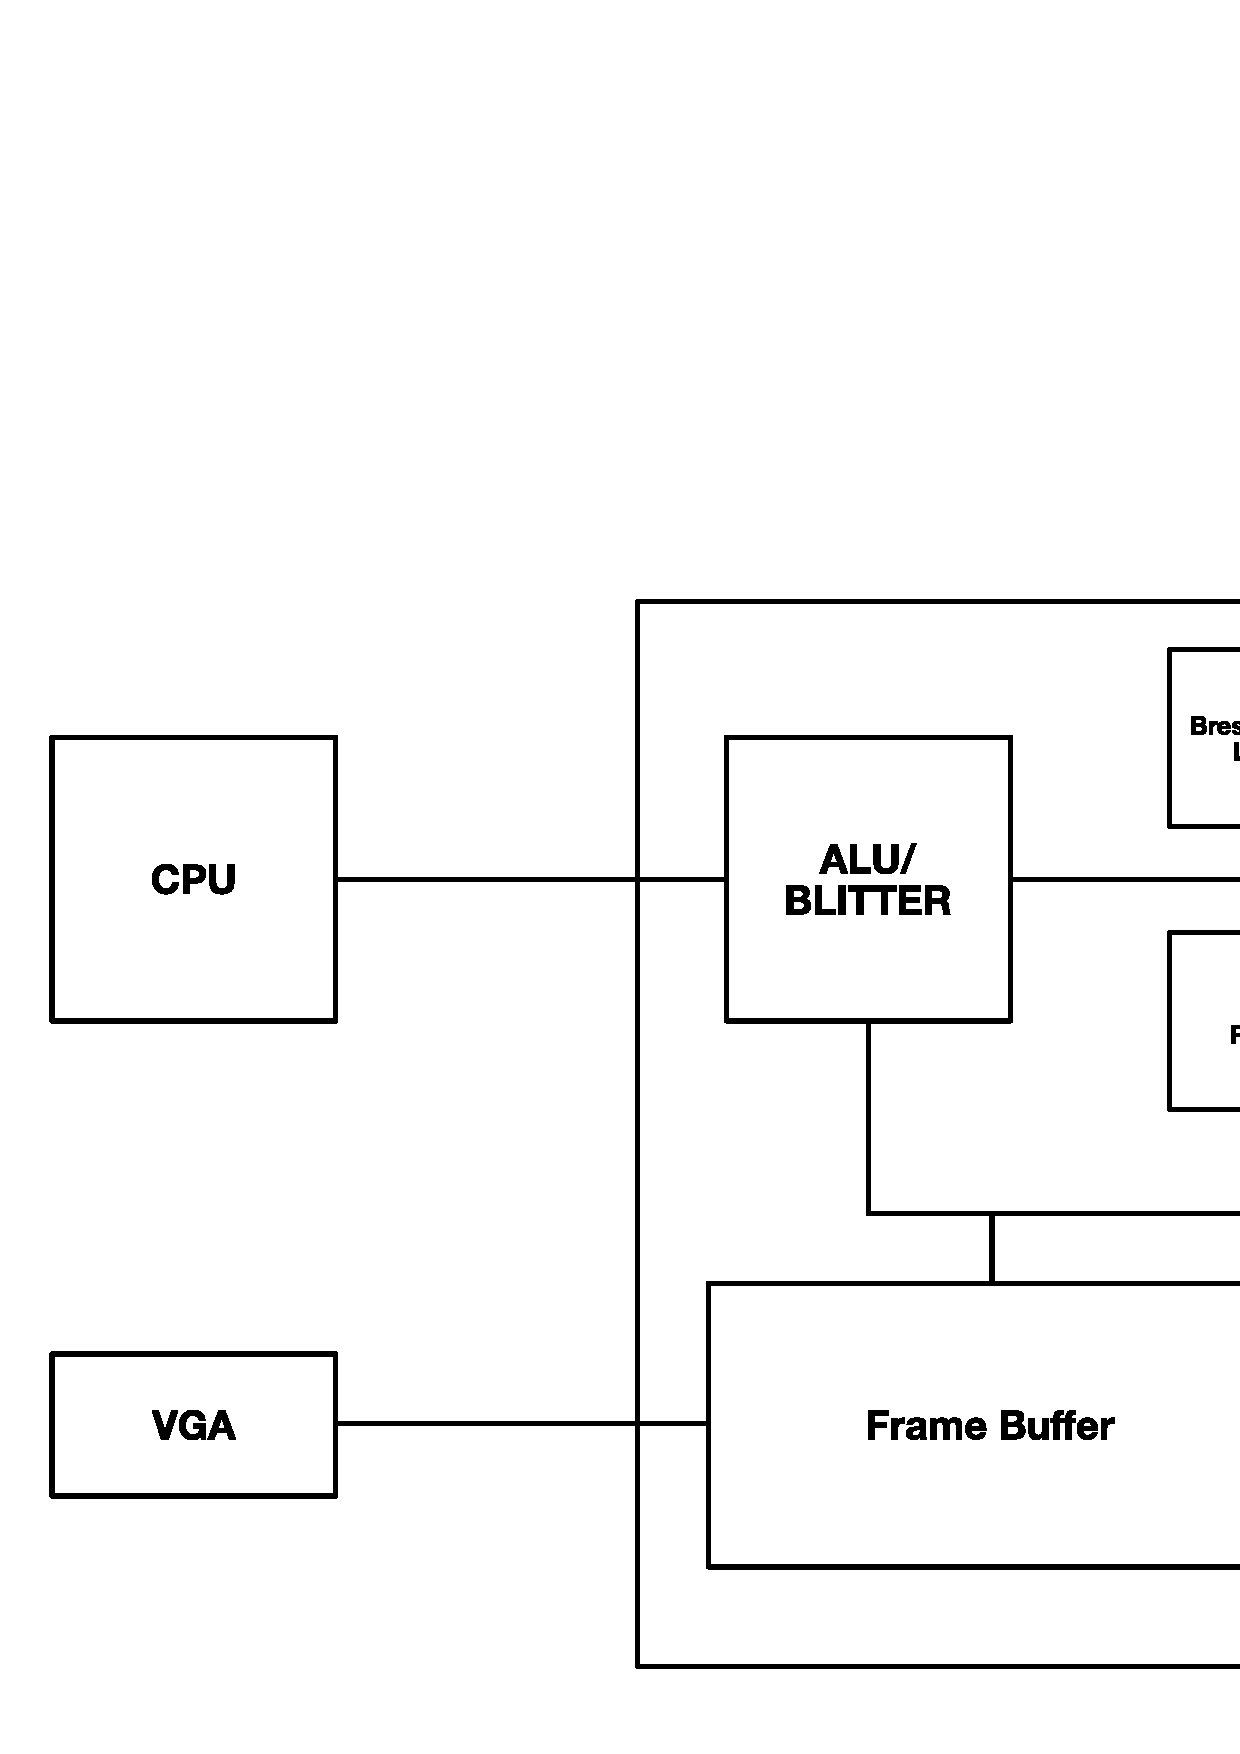
\includegraphics[width=0.5\textwidth]{coredesign}
	\caption{The structure of a GPU pipeline}
	\label{img:gpuPipe}
\end{figure}

The basic structure of how a GPU operates can be seen in \cref{img:gpuPipe}. This pipeline shows the basic functionality of a single core. Each core starts with the processing the vertices. It takes a three dimensional vertex and projects it into screen space, a two dimensional area that gets rendered to the screen. Each vertex is independently projected by a core. In modern computer graphics this process is directed by a vertex shader.

After a vertex is projected into screen space, they are grouped together into logical units that form a triangle. These units are called primitives. They are clipped and culled, where only that is drawn that is visible and facing the screen space, to reduce the processing time needed for the later stages of the pipeline. Those primitives are then rasterized into so called pixel fragments. A pixel fragment is a group of pixels without any color information. To create the color each fragment needs to be shaded to create the visible pixels. Before they are rendered to the screen each fragment is blended into the frame at their pixel location. To determine if a fragment is visible a so called z-buffer is used to determine the drawing order to the frame. This section is handled by a so called fragment shader.

A modern GPU can consist now of up to 2944 such cores \footnote{As taken from \url{https://www.nvidia.com/en-us/geforce/20-series/} on the sixteenth of September of 2019} that all act in somewhat of the previously described functionality.

	
	\subsection{Bresenham Algorithm}
	The original Bresenham Algorithms was developed by J. Bresenham in 1965. The target was to build a algorithm to draw a line between to coordinates on a pixel grid. All the other Bresenham Algorithms that exists, for example to draw a circle are developed by others. In the following section, the Bresenham Line and Circle algorithm were explained.
\subsubsection*{Line Drawing}
The original line algorithm from Bresenham uses only addition, subtraction and a multiplication with two on integer variable. In a Cartesian coordinate system it exist eight variation of a gradient from a line, called octanes. The algorithm uses only one octants. It archived it by transforming the coordinates.

The first step is to set the start coordinate. After that an error variable is set. The error variable is for the decision, which pixel is set next. Is value of the error variable smaller than zero it goes one step in the x direction, is the value bigger equal to zero it goes one step in the y and one step in the x direction. It ends when the new x and y coordinate equals the end x and y coordinate.

(ADD IMAGE HERE FOR BRESENHAM ALGORITHM)

The figure show how the algorithm function. 
\subsubsection*{Circle Drawing}
The circle algorithm function are similar to the line algorithm but it has some differences. One difference is, that it has a circle radius and the coordinate of the middle point of the circle.
	
	\subsection{Bit Blit}\label{sec:blitter}
	\subsubsection*{Moving Data}
Some Text
\subsubsection*{Atari ST and Amiga Blitter}
Some Text
	
	\subsection{Advanced Extensible Interface   4 Bus}
	 
The  advanced microcontroller bus architecture (AMBA) advanced extensible interface 4 (AXI4) is a bus system specified by Advanced RISC Machines (ARM) in the year 2010 \cite{6129797}. The bus system has many features, that why not all feature is described in detail in this chapter.

The AXI4 is a bus that can handle multiple master and slave over intermediate level called interconnect.  
	
	\section{Design and Implementation}
	
	\subsection{Embedded Graphics Accelerator}
	\begin{itemize}
	\item no known modern embedded graphics accelerator
	\item we had to make an open design
	\item not as complex as a regular GPU
	\item more in the lines of a retro gpu like the ones found in an Atari ST or a Commodore Amiga
	\item should take load of the cpu, as the drawing operations would be done by software usually
	\item basic functionality: drawing lines, drawing circles, filling rectangles, drawing font, and drawing in some way a sprite
\end{itemize}
	
	\subsection{VGA and Framebuffer}
	\subsubsection*{Design}
The needs for the implementation were clear from the start of the project. We knew that we are going to need some sort of output to a screen and a framebuffer for an image to be drawn to.

The design of the VGA interface was held flexible, as we wanted the option not only to exchange it with a different interface, but also that we are able to instantiate it with different resolutions. If the FPGA would allow it, a resolution of up to 1080p would be theoretically possible, as it generates its clock from a master clock that is fed in.

The framebuffer is designed to hold two frames at the same time, meaning it is a double buffer. This is something taken from GPU design, as this eliminates the chance of screen tear. This happens when one would want to draw into the image as it is being projected to the screen. Additionally the framebuffer should be instantiated with the maximal size of a frame and its depth of color.

To have the VGA interface and our graphics accelerator access it at the same time, we also decided to give it a true dual port design. As one of the ports is for the VGA interface to read from, while the other port is the the graphics accelerator to read from and write to.
\subsubsection*{Implementation}
\begin{itemize}
	\item the framebuffer object as two read and one write port. 
	\item instanciate with the data it becomes from the VGAConfig
	\item it calculates the size of the mem automaticly. 
	\item first it looks if the resolution is a size of power of two  //code
	\item after that it multiplcate the x and y resolution after that it muliplikate it with two //code
	\item first the vga generate a slow clock area with the frequenc in the VGAConfig
	\item after that it set up some signals and register
	\item the io are connected to the corropending signals
	\item after that some checks are made it y and x counter reaches some special values like end of the line and end of the frame an d picture draw
	\item the buffer control controlls witch buffer the vga can read
	\item the buffer control connects the buffer with the vga and the MCP and here is the logic for the pixel doupler
\end{itemize}
	
	\subsection{Bresenham Line and Circle}\label{subsec:des_bresenham}
	\subsubsection*{Design}
Under the design of the two algorithms of the Bresenham family, we also consider the algorithm for filling rectangles, so everything mentioned for the line and circle also counts for the rectangle. We planned to make all three functions self-sufficient objects, meaning that they could also be used on their own without the thought of a graphics accelerator. Theoretically as they are implemented in hardware they would be able to run in parallel, though the execution on the graphics accelerator is planned to sequential, so that the drawing order can be assured. As there are several renditions of the Bresenham algorithms, we decided to use the most optimized versions, as they lend themselves better for a concurrent execution and were most likely simpler to implement in hardware and as they are designed to draw the most pixels per iteration, in our case this would be on pixel per clock cycle.

\subsubsection*{Implementation}
The inputs and outputs for all three algorithms are rather straight forward. They mainly consist of the input values discussed in \cref{subsec:bres}. As we cannot draw into the negative screen space we decided to create the coordinates as vectors of unsigned integers. This can be seen in \cref{bundline} for the inputs and outputs of the line algorithm. Furthermore we needed a way to trigger the algorithm, which is done with the start boolean. The ready signal tells the rest of the hardware when the algorithm is done and can accept the next values. The last to signals determine the address to where the pixel information is written and if the algorithm is writing pixels at all.
\begin{lstlisting}[language=scala, caption={Line IOs}, label=bundline]
val io = new Bundle {
	val coord1 = in Vec(UInt(1 + log2Up(config.hDisplayBuffer) bits), 
			    		UInt(1 + log2Up(config.vDisplayBuffer) bits))
	val coord2 = in Vec(UInt(1 + log2Up(config.hDisplayBuffer) bits), 
			    		UInt(1 + log2Up(config.vDisplayBuffer) bits))
	val start = in Bool
	val ready = out Bool
	val address = out Vec(UInt(log2Up(config.hDisplayBuffer) bits), 
			      		  UInt(log2Up(config.vDisplayBuffer) bits))
	val setPixel = out Bool
}
\end{lstlisting}
All three algorithms, the line, rectangle and circle, operate with a finite state machine. One such state of this state machine can be seen in \cref{fsmCircle}. This is the idle state. Being the first and initial state of the algorithm, it waits till the start signal is set to high before it starts setting the needed values and calculates certain value. This is done by all three algorithms. After that the line algorithm goes into two state where it calculates the needed error value. This has to be calculated by two states, in the line algorithm, for dependencies reasons, as the error value is dependent on the correct delta values of the x- and y-coordinate. Once the needed variables are calculated the state machine goes into drawing the actual pixels, before it goes back to idle once it is done drawing.
\begin{lstlisting}[language=scala, caption={Start of the Circle Algorithm}, label=fsmCircle]
idle.whenIsActive{
	when (io.start) {
		x1 := io.coord(0)
		y1 := io.coord(1)
		x := (- io.r.asSInt).resized
		y := 0
		err := (2 - (io.r << 1).asSInt).resized
		goto(setPixel1)
	}
}
\end{lstlisting}
The circle algorithm is structured in a similar way as the line algorithm. We can ommit the second coordinate from the line algorithm an replace it with the circle radius. Similarly to the line algorithm it sets and calculates some variables, though it does not need another calculation state, as all the values it needs are done in idle. We the have to draw the four pixels individually, as we have only one write access to the frame buffer. Once it is done with drawing the set of pixels we have to calculate where we have to draw the next. This is done in two calculation states afterwards, similarly to the line algorithm. When it is finished with drawing and calculating it goes back into the idle state.

	
	\subsection{Bit Blit}
	\subsubsection*{Design}
As we want our bit blitter to be nothing more than the memory-to-memory blocking in the Atari ST. We are going to split this process up into two parts. One for the font drawing and one for the sprite drawing, as they have minor differences in how the data looks like.

Both of the will consist of eight by eight pixel information that has to be copied, the difference between them is that the font only consists of an alpha mask, the area which will be drawn, and one color for the letter to be drawn in. The sprite on the other hand has beside the alpha mask, the sprite data that needs to be drawn. This consists of an eight by eight grid of color information. 

\subsubsection*{Implementation}
A separate object is made to copy a letter from the font into the frame buffer. In its state machine we differentiate between the idle state and the copy state, seen in \cref{fontfsm}. When the idle state gets triggered it waits till the start flag is set, similar as in \cref{subsec:des_bresenham}. Once it is triggered to draw it sets a counter to zero and switches into the copy state.
\begin{lstlisting}[language=scala, caption={States of the Font Blitter}, label=fontfsm]
val idle = new State with EntryPoint
val copy = new State
\end{lstlisting}
In the copy state we evaluate each pixel of the alpha mask in a big switch-case. When the value of the pixel is set to high we write the color information for the corresponding pixel. When the whole alpha mask is done, for our case when the counter reaches 63, we go back into the idle state.
to know to which pixel to draw to, the first three bits act as a part of the x-coordinate and the last three bits count for y-coordinate.
\begin{lstlisting}[language=scala, caption={Copying the sprite color information into the frame buffer}, label={blitbuffer}]
for (i <- 4 to 67) {
	is(i) {
		vga.io.wData(0) := buffer(10 downto 0).resized
		vga.io.wData(1) := buffer(21 downto 11).resized
		vga.io.wData(2) := buffer(31 downto 12).resized
		vga.io.wAddress := (!switchVGA 
				  			## (storeVals1(1) + temp(5 downto 3)) 
				  			## (storeVals1(0) + temp(2 downto 0))).asUInt
		vga.io.wValid   := alpha(i - 4)
		counter := counter + 1
		valid := True
		goto(readRam)
	}
}
\end{lstlisting}
The sprite blitter is part of our core, which is discussed in \cref{subsec:core}. The way we have to copy the data functions similarly to how it is done in the font copying. We have to check if the alpha mask is set at a certain pixel. If it is we can draw the pixel of the sprite, this can be seen in \cref{blitbuffer}. Here we also use a switch-case to check the corresponding pixels.

	
	\subsection{AEGIS Core}
	\subsubsection*{Design}
As seen in \cref{img:coredes} the core will consist of a block of memory, an ALU combined with the blitter, and several smaller single function cores.

The graphic accelerator has a double frame buffer. It keeps track of the information of two separate frames. One of the frames is drawn by the VGA module, the other is being created by the graphics accelerator and CPU. The data for the objects are moved into the RAM of the CPU.

As some functions of the blitter correlate with the functions of the ALU (REFERENCE TO AMIGA MANUAL), the two blocks will be merged together in the following the two of them will be referred to as only the ALU. This part of the core will either write directly into the frame buffer or it will delegate the drawing to the proper function core. These smaller function cores consist of the basic graphical primitives, as discussed in \cref{subsec:des_bresenham}.
\begin{figure}[H]
	\centering
	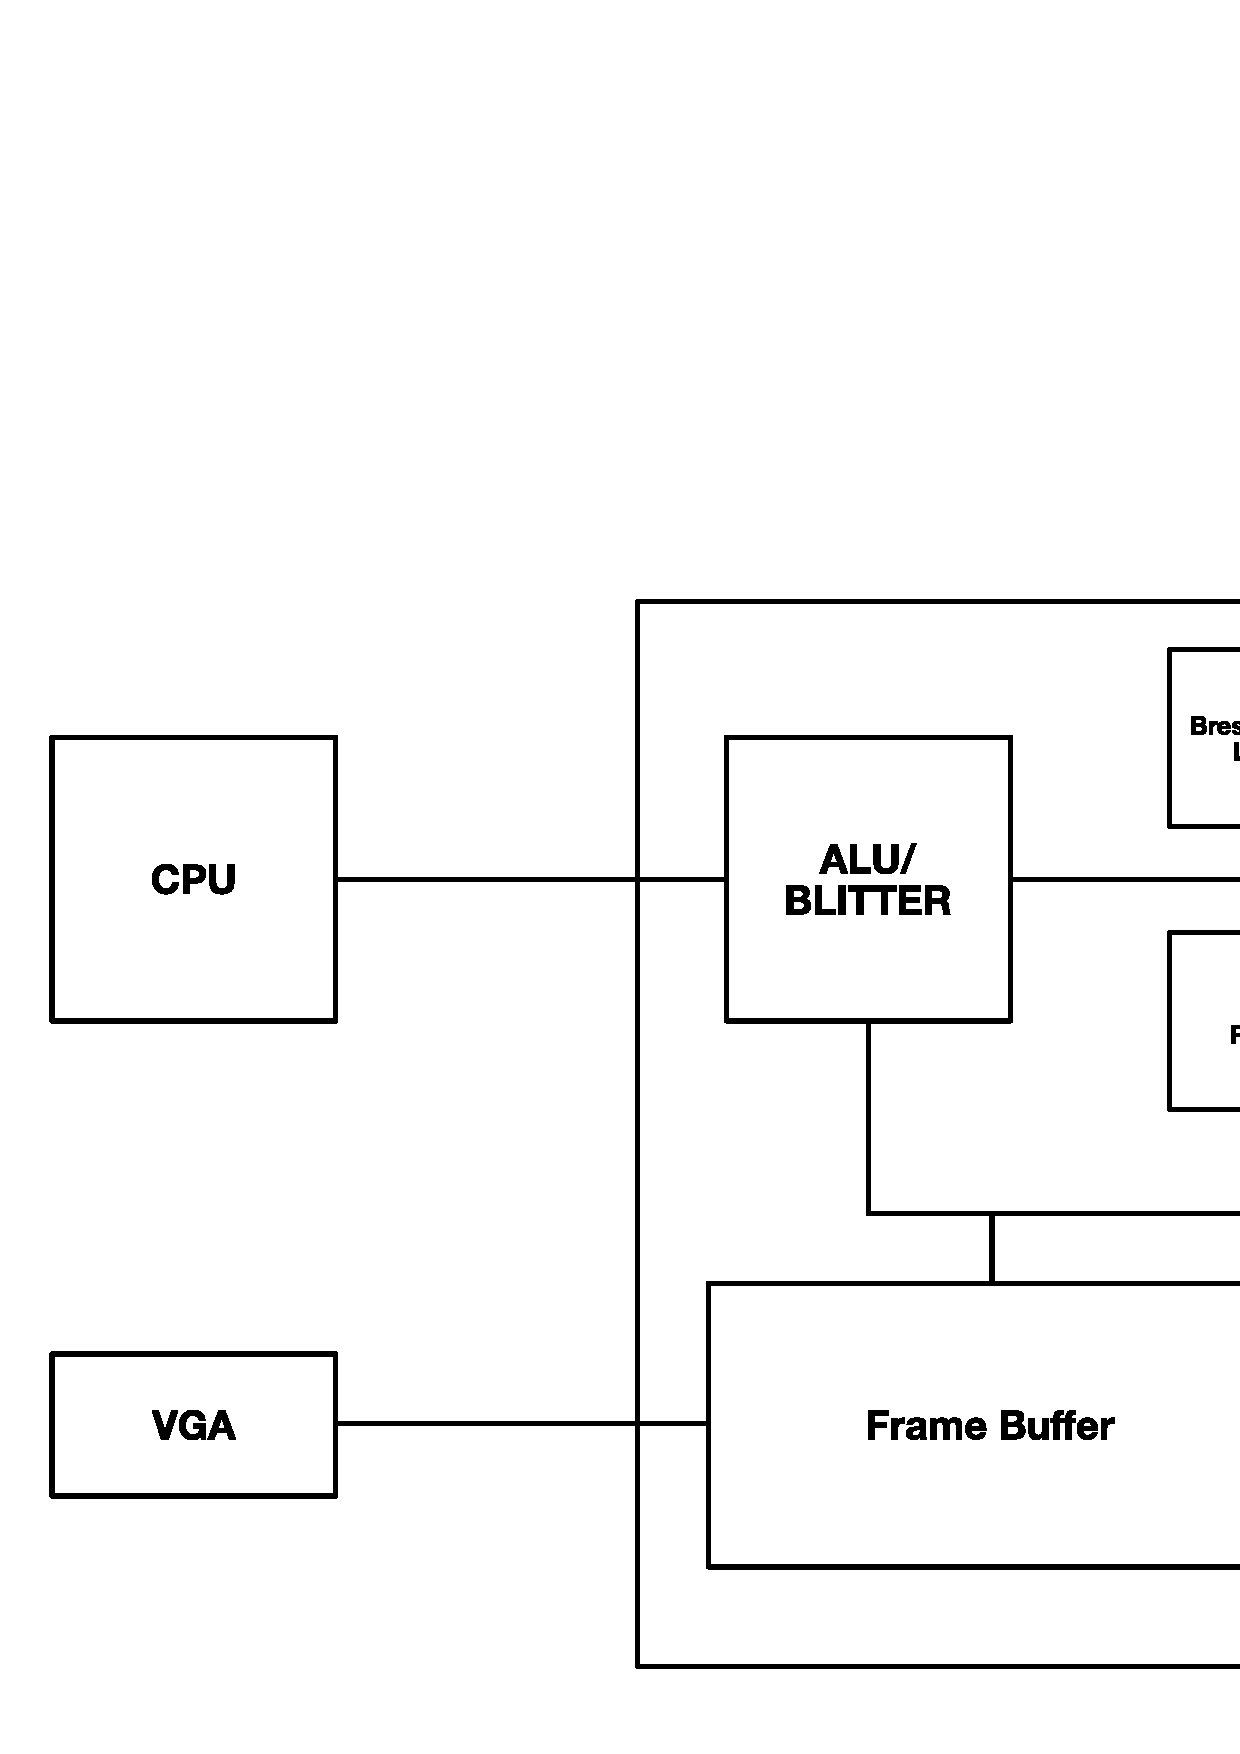
\includegraphics[width=0.5\textwidth]{coredesign}
	\caption{Graphical Design of the AEGIS Core }
	\label{img:coredes}
\end{figure}

For the communication between the CPU and the graphics accelerator, we use two AXI4 buses. The first one is a Axi4Shared for the communication with the CPU, and the second one is a Axi4readonly for the communication with the RAM.

When a write command is send over the AXI4 bus the graphics accelerator looks at the address. Is the address in the range of the double frame buffer, then it writes to it. Otherwise the address determines, what the graphics accelerator do. Further information he needs to operate get it from RAM at the address in the data value. 

\subsubsection*{Implementation}
	
	\subsection{Application Programming Interface}
	\subsubsection*{Design}

During the implementation of the application programming interface (in short API), we had to decide if the user would have to code most of the features from scratch or use the functions we provide for the API.
We decided to choose a mix of both approaches, as we are only giving access to our basic functions of AEGIS. A function of the API should look as follows:
\begin{lstlisting}[language=C, caption={The Circle Drawing Function}, label=CircDraw]
uint32_t ae_draw_circle(uint32_t x, uint32_t y, uint32_t r, Color col);
\end{lstlisting}
The return type of the function indicates, if the function executed successfully (return value \(0\)) or executed with an error (return value greater than \(0\)). To decide if an error occurred or not we would have to read a register flag of the graphics accelerator. A special parameter of the function is the color value. As this should be a 32-bit value, we decided that the user should give us a color as three 32-bit values for each separate color channel as seen in \cref{colStruct}.
\begin{lstlisting}[language=C, caption={The Color Stuct}, label=colStruct]
typedef struct {
	uint32_t red;
	uint32_t green;
	uint32_t blue;
} Color;
\end{lstlisting}

To access the function on the graphics accelerator itself, we plan to use two pointers. One pointer should be used to access the address of the function, while the other one should be used to hold the actual data. 

\subsubsection*{Implementation}

\begin{itemize}
	\item How did it get actually implemented
	\item global pointers to access the single functions of AEGIS
	\item global pointer for the storage of data
	\item implementation of the functions is bare bones, a repeating pattern for every function
	\item return type became legacy code for later implementations
\end{itemize}
	
	\section{Analysis}
	
	
	\section{Conclusion}
	With the results of this project, we have to ask ourselves several question:

\begin{description}
	\item[Did we achive everything planed for the Project?] Unfortunately we had to cut back on some features. We are only able to draw up to eight colors at a resolution of \(320 \times 240\). This is unfortunately the result of the lack of memory on the development boards. If the Altera development boards would have true dual port block memory, then we would have achieved a resolution of up to \(640 \times 480\).
	\item[What was easier than expected?] Two parts were simpler to implement than expected. The Bresenham algorithms fall under this category, as it was almost possible to implement them as they are in software. Also the implementation of the API went quicker than expected, with less errors than expected.
	\item[What was more difficult than expected?] The biggest problem that occurred during the implementation of the graphic accelerator, was the connection to the AXI bus. Not only was it difficult to understand the architecture itself, but also to understand how to use the implementation of the bus for SpinalHDL. This resulted in the most workload of the project.
	\item[Did the results line up with our expectations?] The final results of our project went far and beyond our expectations we had in the beginning of the project. We expected to achieve a frequency of around 45 MHz, which in the end got almost doubled. We also did not expect the difference in cycles needed. We expected more of a factor of between 20 and 30, but not a speedup of up to the factor of 160.
\end{description}


	
	\section{Future Work}
	for a maybe future work paralism (algorithms)
	
	\printbibliography
	
	
\end{document}